\documentclass[a4paper,10 pt]{article}
\usepackage{geometry}
\geometry{letterpaper, margin=0.8in}
\usepackage[english]{babel}
\usepackage[utf8]{inputenc}
\usepackage{amsmath}
\usepackage{graphicx}
\usepackage[colorinlistoftodos]{todonotes}
\usepackage{float}
\usepackage[numbered]{mcode}
\usepackage{hyperref}
\renewcommand{\baselinestretch}{1}

\title{Application of Principal Component Analysis to a Real-World System: An Analysis}

\author{Dana Korssjoen} 

\date{21 February 2020}

\begin{document}
\maketitle
\begin{abstract}
    The intent of this report is to use principal component analysis (PCA) to describe a simple system, comprised of a set of video recordings from multiple angles of a paint can on a string undergoing different types of motion. An object tracking algorithm is first developed, then PCA is applied to better understand the dynamics of the system, then to comment on the methods used to record the data. PCA is found to be a powerful method, especially when facing real-world data that may be rife with redundancies and noise.
\end{abstract}
\section{Introduction and Overview}
This report aims to use the method of principal component analysis to analyze multiple real-world systems, as recorded by multiple cameras at different angles. An algorithm to track the object of interest is first developed, then principal component analysis is applied to the derived positions to describe the motion of the object of interest. The results facilitate a discussion of redundancy in the recording methods, as well as of the practice and implications of the PCA method as a whole.

Each section of this report describes a crucial part of the project implementation, starting from theoretical background, moving into algorithm development, then discussing computational results and their implications. The appendix contains the Matlab code used to generate this analysis, should an interested reader want to recreate the results.

\section{Theoretical Background}
\subsection{Singular Value Decomposition (SVD)}
The singular value decomposition is the process of decomposing a matrix into the form \begin{equation}
    \mathbf{A} = \mathbf{U\Sigma V^*}
\end{equation}
Each component in this equation will now be discussed in more depth. The first two are $\mathbf{U}$, which is a unitary, square matrix with dimensions equal to the number of rows in the matrix $\mathbf{A}$, and $\mathbf{V}$, which is a unitary square matrix with dimensions equal to the number of columns (i.e. observations) in $\mathbf{A}$. Both of these matrices are orthonormal bases that can be used to expand any vector which occupies their respective spaces (which are the range and domain of $\mathbf{A}$, respectively). In fact, any matrix $\mathbf{A}$ has a singular value decomposition, as any vector can be expressed as a combination of the components given in this fundamental equation.

The next component is $\mathbf{\Sigma}$, which is a diagonal matrix. Moreover, its entries are sorted in descending order. These entries are called the singular values of matrix $\mathbf{A}$, and they represent what share of the total information contained in $\mathbf{A}$ is captured by the corresponding mode. One would anticipate a redundant data set, or one with very few degrees of freedom, to have very few large singular values.

\subsection{Principal Component Analysis (PCA)}
We know turn to principal component analysis, which is an application of the SVD. It is particularly useful to study unknown, but potentially low-dimensional systems. It is popular for real-world data, because it is well-suited to handle noisy or redundant data sets. The reason for this is that PCA describes the principal dynamics of a system, thus reducing the impact of noise; and it can be used to describe the statistical dependence of two data sets, called covariance. Concretely, if we have two vectors $\mathbf{a}$ and $\mathbf{b}$ of observations, we compute their respective variance by
\begin{equation}
    \sigma^2_a = \frac{1}{n-1}\mathbf{aa}^T\quad\quad\sigma^2_b = \frac{1}{n-1}\mathbf{bb}^T,
\end{equation}
and their covariance by
\begin{equation}
    \sigma^2_{ab} = \frac{1}{n-1}\mathbf{ab}^T,
\end{equation}
where $1/(n-1)$ is used to reduce bias. If we have many vectors of observations, we may combine them in a single matrix $\mathbf{X}$ and find their covariance by
\begin{equation}
    \mathbf{C_X} = \frac{1}{n-1}\mathbf{XX}^T.
\end{equation}

The reason that this ties into SVD is that we can diagonalize the covariance matrix by computing the variance in $\mathbf{Y}$, called the \emph{principal component projection} of $\mathbf{X}$, computed by the following equation
\begin{equation}
    \mathbf{Y} = \mathbf{U^*X}.
\end{equation}
We then find the covariance using the properties of this matrix as follows:
\begin{equation}
    \mathbf{C_Y} = \frac{1}{n-1}\mathbf{YY}^T = \frac{1}{n-1}(\mathbf{U^*X})(\mathbf{U^*X})^T = \frac{1}{n-1}\mathbf{U}^*\mathbf{U}\mathbf{\Sigma}^2\mathbf{UU}^* = \frac{1}{n-1}\mathbf{\Sigma}^2,
\end{equation}
and so we know that we can compute the covariance using the singular value decomposition.

In this way, we can find the principal components of a system, control the influence of redundancy, and precisely describe what share of the total energy of the system each component represents. With that background established, we are ready to discuss the algorithms used in this report.

\section{Algorithm Implementation and Development}
\subsection{Position Tracking}
The script used to track the position of the paint can in the video is in Appendix B, lines 1-75. Here, ``position'' is defined as the visual center of the paint can in the frame, which is manually defined by the user in frame 1 of each video.

This script contains calls to getPos(), which is the position tracking function used in this report. That algorithm is explained in detail later in this section.

After obtaining the initial x-y position matrices, the matrices for each camera in each case are trimmed to be a constant length across each case, and to start at approximately the same time, achieved by trimming each matrix so that it began with the first point at which the y-displacement was at a minimum. Synchronizing the data in this way allows us to knit each case into a single matrix that contains all 3 camera angles, which is crucial for the application of PCA.

On lines 77-253, PCA is performed and the graphs shown in this report are generated. We will focus on lines 78-112, which perform these steps for case 1; the other cases have analogous code. The code is lengthy, but not complex. To perform PCA, the row means are subtracted from the data set to give each row a mean of 0, then PCA is performed as described in the theoretical background. The singular values are used to compute and graph the energy contained in each mode, and the projections of the data onto the first 3 modes are graphed, as well.

Lines 255-296 contain the functions used to track the object's position. The main wrapper function is getPos(), which takes in a video, allows the user to input the initial position of the object, and then calls tracker() to find its position in each subsequent frame. After this, it returns the matrix of x-y positions where each column corresponds to a frame in the video. The bulk of the work is done by tracker(), which essentially uses a moving ``box'' to track the object in the video. Specifically, it takes as input the contents of the box from the prior frame, in which the object is centered, and it chooses the new box that minimizes the sum of squared errors between their contents - that is, the box with the most similar image contained inside of it. It chooses candidates by testing boxes centered at each pixel in the search box defined by the given radius, then choosing the best box. The center of that box is returned as the position of the object at that time. For best results, the box should be approximately the size of the object in the frame - the value of 20 was chosen experimentally.

The function getBox() is simply a helper function that computes the prior frame's box (as chosen by tracker()), in which the object is centered.

\section{Computational Results}
Note that for brevity, not every figure generated by the included Matlab code is demonstrated in this report, though the most important concepts are well-illustrated.
\subsection{Case I: Simple Harmonic Motion}
In this set of videos, the paint can was simply oscillating up and down in what can be described as simple harmonic motion. Noise from camera shake was minimized in the recording process. This can be seen in Figure 1, where the vertical displacement over time (as described by discrete videos frames) is graphed. In the figure, it is clear that even though the object occupied a different spot in the frame of each of the camera angles, its motion was synchronized. The graph is notably without noise or other irregularities.

Figure 2 demonstrates the result of applying PCA to the system. In the top graph, which depicts the percentage of total energy captured by each mode, it is clear that the 1-mode approximation is more than sufficient, capturing nearly 100\% of total energy. Still, the projection of the data onto the first 3 modes is depicted for completeness. Notice that mode displays exactly the sort of simple harmonic motion that we would expect for this system. The fact that almost the entirety of the energy was contained in mode 1 suggests that one well-placed camera would have been sufficient to record the dynamics of this system.
\begin{figure}[H]
  \centering
    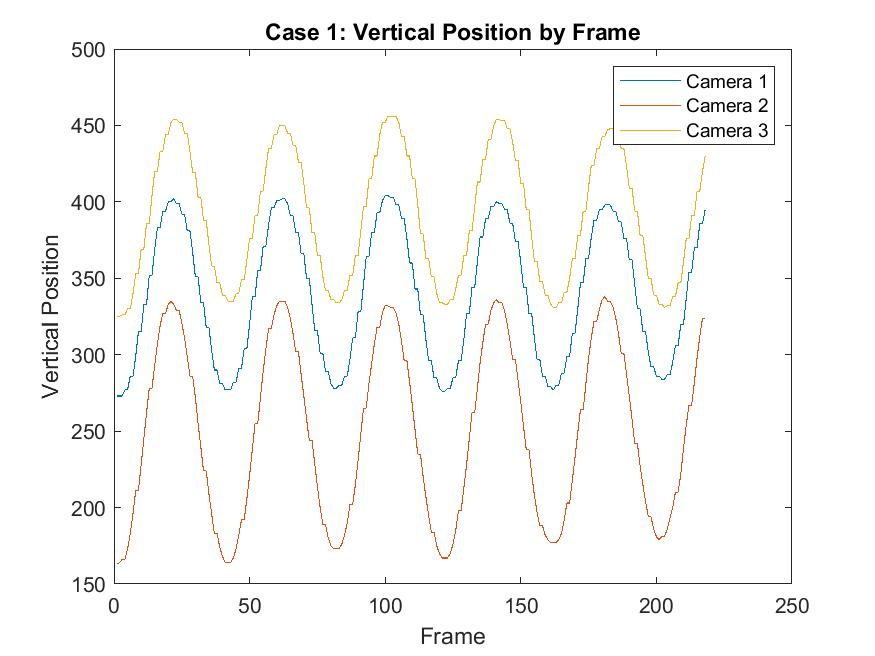
\includegraphics[width = 0.5\textwidth]{hw3/images/case1-y-pos.jpg}
    \caption{Tracked Motion in Case I}
\end{figure}

\begin{figure}[H]
  \centering
    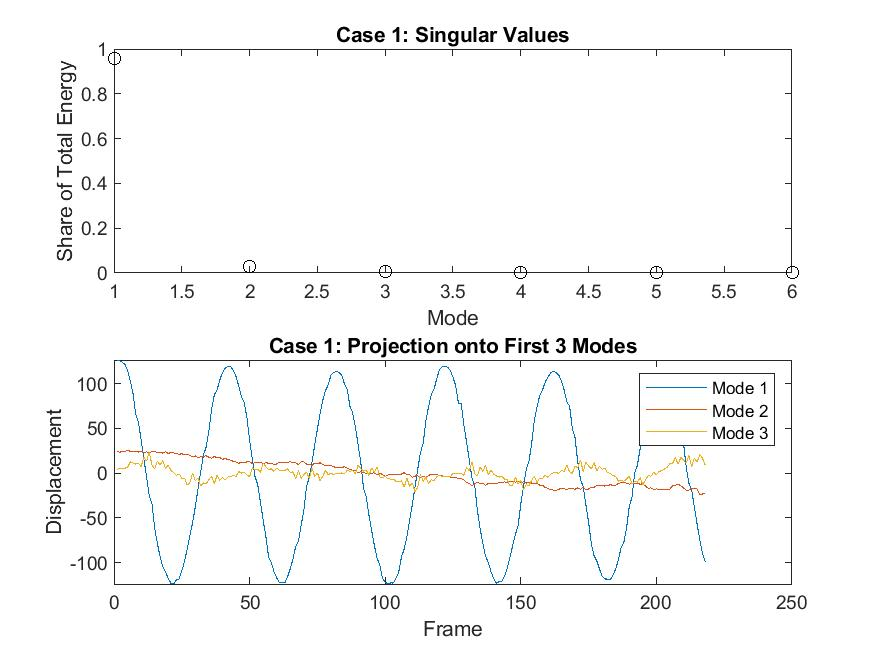
\includegraphics[width = 0.5\textwidth]{hw3/images/case1-modes.jpg}
    \caption{Results of PCA on Case I}
\end{figure}

\subsection{Case II: Simple Harmonic Motion with Noise}
This case is much like Case I, in that we have only simple harmonic motion, however noise is also introduced in the form of camera shake. We can see this in Figure 3, where we would expect to see relatively constant horizontal positions for a system with only vertical displacement, but significant horizontal movement is observed. As displayed in Figure 4, this introduces more complexity to the PCA of the system, though the vast majority of energy is still captured by mode 1, and mode 2 is noticeably sinusoidal.

\begin{figure}[H]
  \centering
    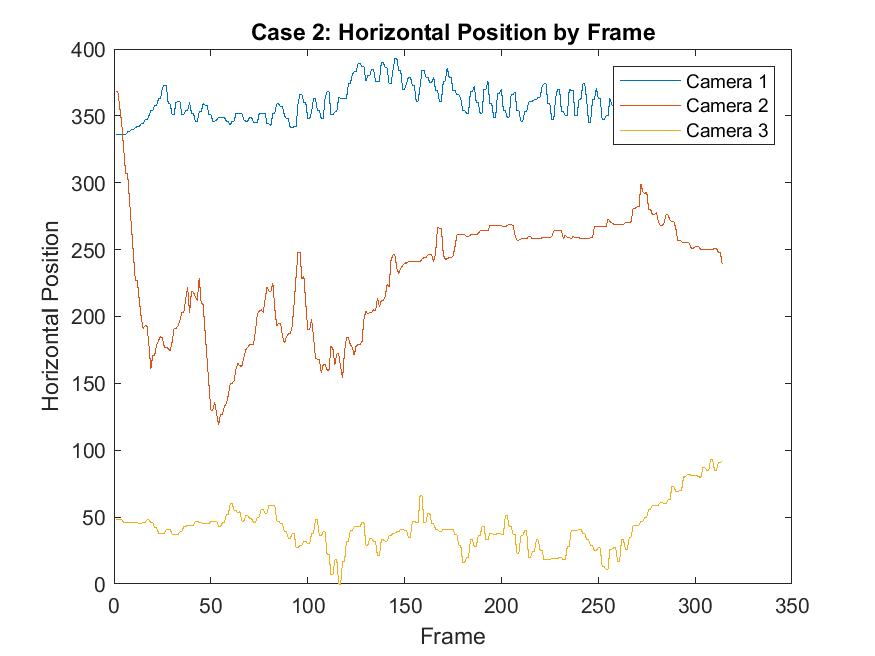
\includegraphics[width = 0.5\textwidth]{hw3/images/case2-x-pos.jpg}
    \caption{Tracked Motion in Case II}
\end{figure}

\begin{figure}[H]
  \centering
    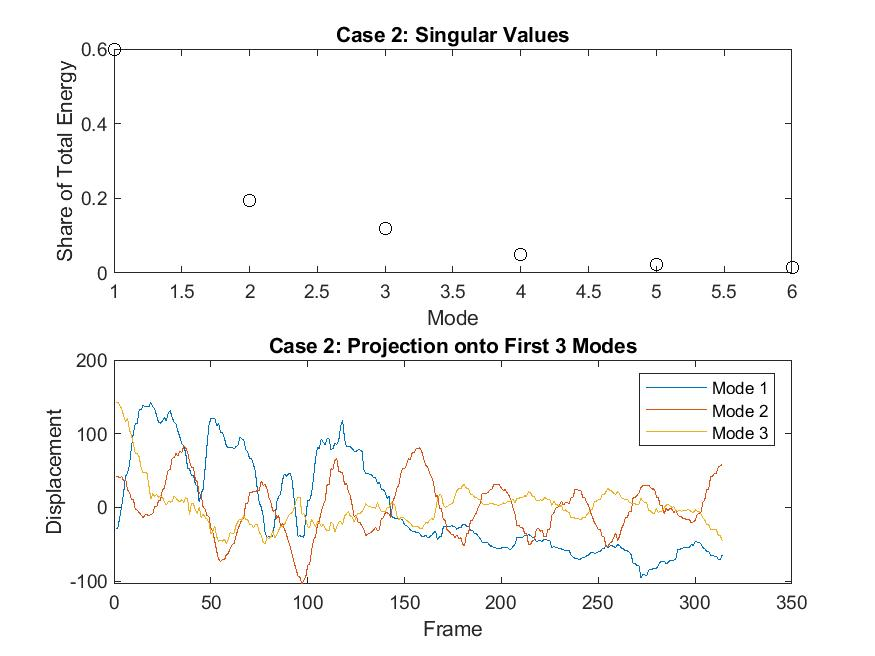
\includegraphics[width = 0.5\textwidth]{hw3/images/case2-modes.jpg}
    \caption{Results of PCA on Case II}
\end{figure}

\subsection{Case III: Harmonic Motion with Pendulum Motion}
In this case, we introduce pendulum motion to the prior system, so that our object is now moving both up and down (simple harmonic motion) and back and forth (pendulum motion). The ``back and forth'' dynamics are in Figure 5. As anticipated, this results in a PCA where both modes 1 and 2 are sinusoidal, representing harmonic motion in two orthonormal bases. Notice also that mode 3 captures a significant amount of energy, suggesting that 3 cameras would be an appropriate choice for this system.

\begin{figure}[H]
  \centering
    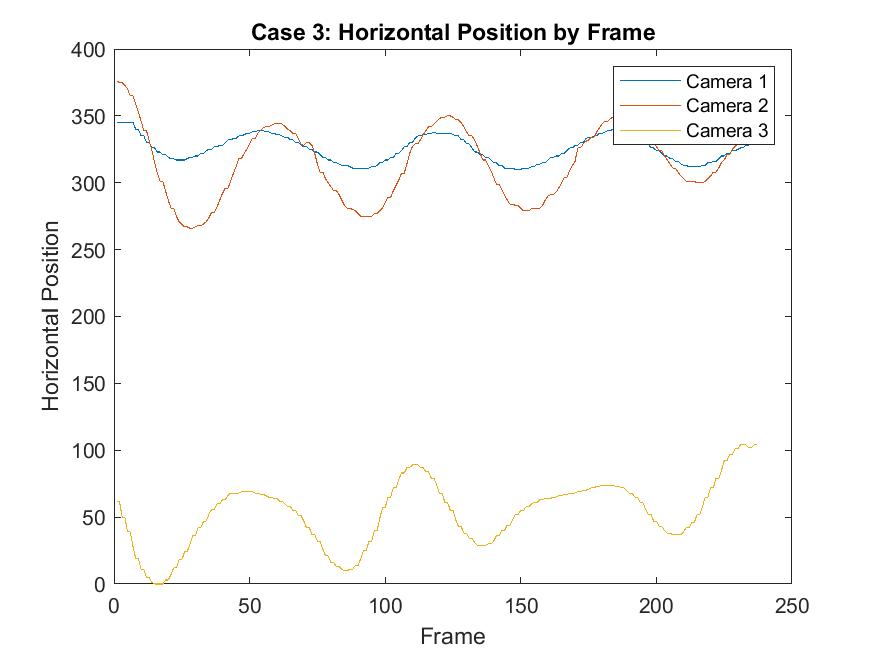
\includegraphics[width = 0.5\textwidth]{hw3/images/case3-x-pos.jpg}
    \caption{Tracked Motion in Case III}
\end{figure}

\begin{figure}[H]
  \centering
    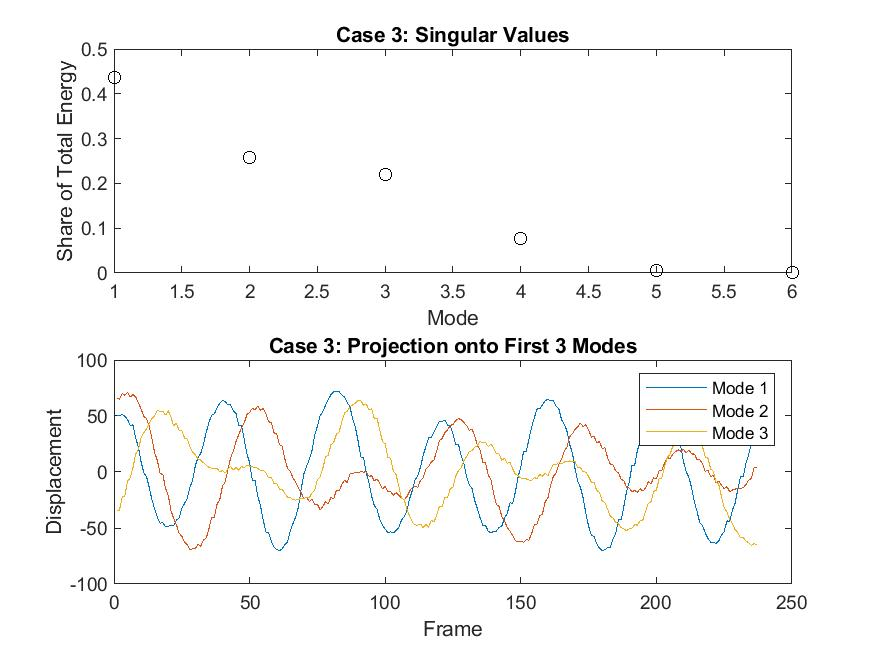
\includegraphics[width = 0.5\textwidth]{hw3/images/case3-modes.jpg}
    \caption{Results of PCA on Case III}
\end{figure}

\subsection{Case IV: Harmonic Motion, Pendulum Motion, and Rotation}
In this case, we have all of the dynamics of previous cases with rotation introduced. Note that this doesn't affect the system significantly due to our choice of object tracking algorithm, which tracks the visual center of the object in the frame, rather than a fixed point on it. Note also that for space reasons, the motion captured in this case have been omitted, but the PCA is still included for the purpose of discussion.

In Figure 7, we see a graph very similar to the one observed for Case III, with slightly more energy contained in later modes than before. This makes sense, as we have introduced another type of motion (rotation), but as mentioned, it does not factor significantly into our object tracking algorithm, so it does not affect the system drastically.
\begin{figure}[H]
  \centering
    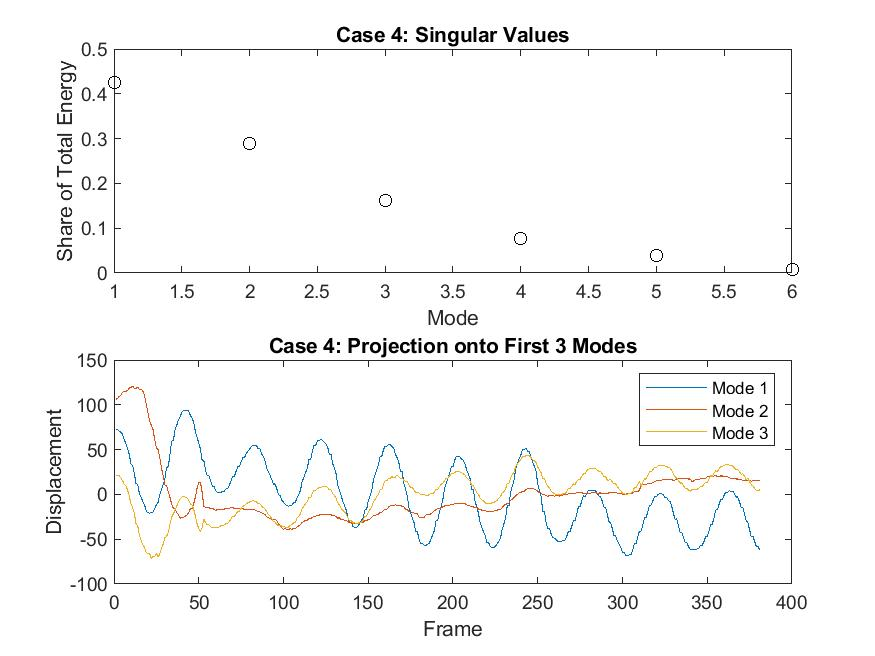
\includegraphics[width = 0.5\textwidth]{hw3/images/case4-modes.jpg}
    \caption{Results of PCA on Case IV}
\end{figure}

\section{Summary and Conclusions}
In this report, the theory, practice, and implications of PCA have been discussed and applied to a real-world case study. The method was found to be remarkably powerful at describing redundancies in a data set, as well as handling noise introduced by the recording process. The dominant motion of all of the systems was captured in all 4 cases by PCA, and we were able to speak with confidence about the difference in dynamics between the systems, having quantifiable indicators for their differences. Altogether, this is a powerful data analysis tool which is apt to be applied to real-world data on low-dimensional, possibly unknown systems.
\section{Appendix A: MATLAB Functions and Implementation}
See Table 1, above.
\begin{table}[]
\begin{tabular}{ll}
load() & loads the data stored in the given file \\
max() & finds the maximum value in the given data structure \\
size() & returns the size of the given data structure, with optional dimension arguments \\
min() & finds the minimum value in the given data structure \\
save('file\_name','obj\_name') & saves the specified object as a file with the given name \\
mean() & calculates the mean of the given object \\
repmat(A,n) & returns a matrix with n copies of object A \\
svd() & performs singular value decomposition on the given matrix \\
diag() & returns a vector of the diagonal elements of the given matrix \\
subplot(m,n,k) & creates a plot grid with m rows and n columns, then plots the current figure on the plot with the linear subscript k \\
xlabel()/ylabel() & writes the given label to a plot along the given dimension \\
title()/legend() & writes the given title or legend entries to the current plot \\
zeros() & creates a matrix of zeros with the given dimensions \\
imshow() & displays the given image \\
ginput(n) & stores the location of n user-inputted clicks on the current figure \\
int16() & casts the given data structure to the int16 type
\end{tabular}
\caption{Matlab Commands and their Meanings}
\end{table}
\section{Appendix B: MATLAB Code}
\begin{lstlisting}
%% create position vectors
% generate initial vectors
load('cam1_1.mat');
pos1_1 = getPos(vidFrames1_1);
load('cam2_1.mat');
pos2_1 = getPos(vidFrames2_1);
load('cam3_1.mat');
pos3_1 = getPos(vidFrames3_1);

load('cam1_2.mat');
pos1_2 = getPos(vidFrames1_2);
load('cam2_2.mat');
pos2_2 = getPos(vidFrames2_2);
load('cam3_2.mat');
pos3_2 = getPos(vidFrames3_2);

load('cam1_3.mat');
pos1_3 = getPos(vidFrames1_3);
load('cam2_3.mat');
pos2_3 = getPos(vidFrames2_3);
load('cam3_3.mat');
pos3_3 = getPos(vidFrames3_3);
load('cam1_4.mat');
pos1_4 = getPos(vidFrames1_4);
load('cam2_4.mat');
pos2_4 = getPos(vidFrames2_4);
load('cam3_4.mat');
pos3_4 = getPos(vidFrames3_4);

% trim and synchronize data
pos3_1 = [max(pos3_1(2,:))-pos3_1(2,:);pos3_1(1,:)]; % rotate cam 3
pos1_trimmed = pos1_1(:,9:size(pos1_1,2));
pos2_trimmed = pos2_1(:,19:size(pos2_1,2));
pos3_trimmed = pos3_1(:,8:size(pos3_1,2));
minLength = min([size(pos1_trimmed,2),size(pos2_trimmed,2),size(pos3_trimmed,2)]);
pos1_trimmed = pos1_trimmed(:,1:minLength);
pos2_trimmed = pos2_trimmed(:,1:minLength);
pos3_trimmed = pos3_trimmed(:,1:minLength);
knit1 = [pos1_trimmed; pos2_trimmed; pos3_trimmed];

pos3_2 = [max(pos3_2(2,:))-pos3_2(2,:);pos3_2(1,:)]; % rotate cam 3
pos1_trimmed = pos1_2(:,1:size(pos1_2,2));
pos2_trimmed = pos2_2(:,16:size(pos2_2,2));
pos3_trimmed = pos3_2(:,1:size(pos3_2,2));
minLength = min([size(pos1_trimmed,2),size(pos2_trimmed,2),size(pos3_trimmed,2)]);
pos1_trimmed = pos1_trimmed(:,1:minLength);
pos2_trimmed = pos2_trimmed(:,1:minLength);
pos3_trimmed = pos3_trimmed(:,1:minLength);
knit2 = [pos1_trimmed; pos2_trimmed; pos3_trimmed];

pos3_3 = [max(pos3_3(2,:))-pos3_3(2,:);pos3_3(1,:)];
pos1_trimmed = pos1_3(:,1:size(pos1_3,2));
pos2_trimmed = pos2_3(:,25:size(pos2_3,2));
pos3_trimmed = pos3_3(:,1:size(pos3_3,2));
minLength = min([size(pos1_trimmed,2),size(pos2_trimmed,2),size(pos3_trimmed,2)]);
pos1_trimmed = pos1_trimmed(:,1:minLength);
pos2_trimmed = pos2_trimmed(:,1:minLength);
pos3_trimmed = pos3_trimmed(:,1:minLength);
knit3 = [pos1_trimmed; pos2_trimmed; pos3_trimmed];

pos3_4 = [max(pos3_4(2,:))-pos3_4(2,:);pos3_4(1,:)];
pos1_trimmed = pos1_4(:,12:size(pos1_4,2));
pos2_trimmed = pos2_4(:,21:size(pos2_4,2));
pos3_trimmed = pos3_4(:,10:size(pos3_4,2));
minLength = min([size(pos1_trimmed,2),size(pos2_trimmed,2),size(pos3_trimmed,2)]);
pos1_trimmed = pos1_trimmed(:,1:minLength);
pos2_trimmed = pos2_trimmed(:,1:minLength);
pos3_trimmed = pos3_trimmed(:,1:minLength);
knit4 = [pos1_trimmed; pos2_trimmed; pos3_trimmed];

% save knitted matrices
save('knit1.mat','knit1');
save('knit2.mat','knit2');
save('knit3.mat','knit3');
save('knit4.mat','knit4');

%% perform PCA and generate graphs
% case 1
load('knit1.mat')
n = size(knit1,2);
means = mean(knit1,2);
kn = knit1 - repmat(means,1,n); % norm means
[U,S,V] = svd(kn/sqrt(n-1));
lambda = diag(S).^2;
Y = U'*kn; % calculate PC projection

subplot(2,1,1)
plot(lambda/sum(lambda),'ko')
xlabel('Mode')
ylabel('Share of Total Energy')
title('Case 1: Singular Values')

subplot(2,1,2)
t = 1:n;
plot(t, Y(1,:), t, Y(2,:), t, Y(3,:))
xlabel('Frame')
ylabel('Displacement')
title('Case 1: Projection onto First 3 Modes')
legend('Mode 1','Mode 2','Mode 3')
saveas(gcf,'case1-modes.jpg')

% y-motion
frames1 = 1:size(knit1,2);
plot(frames1,knit1(2,:))
hold on
plot(frames1,knit1(4,:));
plot(frames1,knit1(6,:));
title('Case 1: Vertical Position by Frame')
xlabel('Frame')
ylabel('Vertical Position')
legend('Camera 1','Camera 2','Camera 3')
saveas(gcf,'case1-y-pos.jpg')

% case 2
load('knit2.mat')
n = size(knit2,2);
means = mean(knit2,2);
kn = knit2 - repmat(means,1,n); % norm means
[U,S,V] = svd(kn/sqrt(n-1));
lambda = diag(S).^2;
Y = U'*kn; % calculate PC projection

subplot(2,1,1)
plot(lambda/sum(lambda),'ko')
xlabel('Mode')
ylabel('Share of Total Energy')
title('Case 2: Singular Values')

subplot(2,1,2)
t = 1:n;
plot(t, Y(1,:), t, Y(2,:), t, Y(3,:))
xlabel('Frame')
ylabel('Displacement')
title('Case 2: Projection onto First 3 Modes')
legend('Mode 1','Mode 2','Mode 3')
saveas(gcf,'case2-modes.jpg')

% y-motion
frames1 = 1:size(knit2,2);
plot(frames1,knit2(2,:))
hold on
plot(frames1,knit2(4,:));
plot(frames1,knit2(6,:));
title('Case 2: Vertical Position by Frame')
xlabel('Frame')
ylabel('Vertical Position')
legend('Camera 1','Camera 2','Camera 3')
saveas(gcf,'case2-y-pos.jpg')

% x motion
plot(frames1,knit2(1,:))
hold on
plot(frames1,knit2(3,:));
plot(frames1,knit2(5,:));
title('Case 2: Horizontal Position by Frame')
xlabel('Frame')
ylabel('Horizontal Position')
legend('Camera 1','Camera 2','Camera 3')
saveas(gcf,'case2-x-pos.jpg')

% case 3
load('knit3.mat')
n = size(knit3,2);
means = mean(knit3,2);
kn = knit3 - repmat(means,1,n); % norm means
[U,S,V] = svd(kn/sqrt(n-1));
lambda = diag(S).^2;
Y = U'*kn; % calculate PC projection

subplot(2,1,1)
plot(lambda/sum(lambda),'ko')
xlabel('Mode')
ylabel('Share of Total Energy')
title('Case 3: Singular Values')

subplot(2,1,2)
t = 1:n;
plot(t, Y(1,:), t, Y(2,:), t, Y(3,:))
xlabel('Frame')
ylabel('Displacement')
title('Case 3: Projection onto First 3 Modes')
legend('Mode 1','Mode 2','Mode 3')
saveas(gcf,'case3-modes.jpg')

% y-motion graphs
frames1 = 1:size(knit3,2);
plot(frames1,knit3(2,:))
hold on
plot(frames1,knit3(4,:));
plot(frames1,knit3(6,:));
title('Case 3: Vertical Position by Frame')
xlabel('Frame')
ylabel('Vertical Position')
legend('Camera 1','Camera 2','Camera 3')
saveas(gcf,'case3-y-pos.jpg')

% x motion
plot(frames1,knit3(1,:))
hold on
plot(frames1,knit3(3,:));
plot(frames1,knit3(5,:));
title('Case 3: Horizontal Position by Frame')
xlabel('Frame')
ylabel('Horizontal Position')
legend('Camera 1','Camera 2','Camera 3')
saveas(gcf,'case3-x-pos.jpg')

% case 4
load('knit4.mat')
n = size(knit4,2);
means = mean(knit4,2);
kn = knit4 - repmat(means,1,n); % norm means
[U,S,V] = svd(kn/sqrt(n-1));
lambda = diag(S).^2;
Y = U'*kn; % calculate PC projection

subplot(2,1,1)
plot(lambda/sum(lambda),'ko')
xlabel('Mode')
ylabel('Share of Total Energy')
title('Case 4: Singular Values')

subplot(2,1,2)
t = 1:n;
plot(t, Y(1,:), t, Y(2,:), t, Y(3,:))
xlabel('Frame')
ylabel('Displacement')
title('Case 4: Projection onto First 3 Modes')
legend('Mode 1','Mode 2','Mode 3')
saveas(gcf,'case4-modes.jpg')

% y-motion graphs
frames1 = 1:size(knit4,2);
plot(frames1,knit4(2,:))
hold on
plot(frames1,knit4(4,:));
plot(frames1,knit4(6,:));
title('Case 4: Vertical Position by Frame')
xlabel('Frame')
ylabel('Vertical Position')
legend('Camera 1','Camera 2','Camera 3')
saveas(gcf,'case4-y-pos.jpg')

% x motion
plot(frames1,knit4(1,:))
hold on
plot(frames1,knit4(3,:));
plot(frames1,knit4(5,:));
title('Case 4: Horizontal Position by Frame')
xlabel('Frame')
ylabel('Horizontal Position')
legend('Camera 1','Camera 2','Camera 3')
saveas(gcf,'case4-x-pos.jpg')

%% getPos.m
function pos = getPos(video)
    pos = zeros(2,size(video,4));
    imshow(video(:,:,:,1));
    pos(:,1) = int16(ginput(1));
    for j = 2:size(video,4)
        lastBox = getBox(video(:,:,:,j-1), pos(:,j-1), 20, 20);
        pos(:,j) = tracker(video(:,:,:,j), lastBox, pos(:,j-1), 20, 20);
    end
end

%% tracker.m
function pos = tracker(frame, lastBox, prev, boxR, searchR)
    min_error = 1e10; % larger than any possible error
    minX = max(boxR+1, prev(1)-searchR);
    maxX = min(size(frame,2)-boxR, prev(1)+searchR);
    minY = max(boxR+1, prev(2)-searchR);
    maxY = min(size(frame,1)-boxR, prev(2)+searchR);
    for x = minX:maxX
        for y = minY:maxY
            % find best new box
            newBox = frame((y-boxR):(y+boxR),(x-boxR):(x+boxR),:);
            error = sum((int16(newBox) - int16(lastBox)).^2,'all');
            if error < min_error
               min_error = error;
               min_point = [x;y];
            end
        end
    end
    pos = min_point;
end

%% getBox.m
function box = getBox(frame, prev, boxR, searchR)
    minX = max(boxR+1, prev(1)-searchR);
    maxX = min(size(frame,2)-boxR, prev(1)+searchR);
    
    minY = max(boxR+1, prev(2)-searchR);
    maxY = min(size(frame,1)-boxR, prev(2)+searchR);
    
    box = frame(minY:maxY,minX:maxX,:);
end
\end{lstlisting}
\end{document}